\chapter[Requirements, Design, and Implementation]{Requirements, Design, And\\ Implementation}\label{ch:ReqDesignImp}
\section{Requirements}
Based upon group discussions in a classroom setting, it was decided what information that the Collection Management team would provide to the other teams that need to work with cleaned tweet data. A full specification of these decisions can be found by viewing the Collection Management team's report; however we will briefly discuss the points that were relevant to us.

Given the cleaned tweet data from Collection Management, our team will be able to perform the methodologies we describe later to classify whether a document is relevant or non-relevant to a given class. A detailed layout of the project with our interactions highlighted is provided by Figure \ref{fig:design}.

We will then place our classification information in the HBase datastore to mark the relevance of each document. The Solr team will index this class information that we provide, allowing for more robust query results and more useful facets to be created.

\begin{figure}[ht]
	\centering
	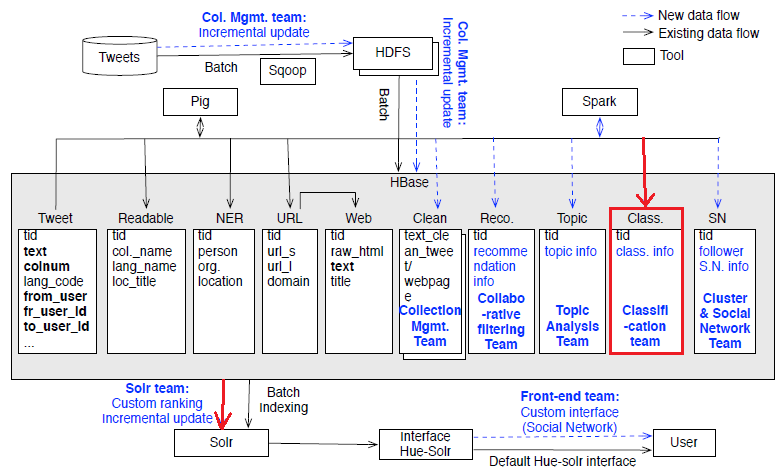
\includegraphics[width=\textwidth]{figures/data_flow.png}
    \caption{Layout of the project teams, as provided by Professor Fox and his GRAs.}\label{fig:design}
\end{figure}

\section{Design}
Our current design is based primarily off of recommendations from the GRAs assisting the class. We have also taken substantial input from last year's Classification team \cite{cui2015classification} and the Professor.

We have designed our current solution around pulling training data from and testing on a small collection of around 100,000 tweets. This was originally going to be performed on the small collection that was assigned to our team, \texttt{\#germanwings}. However, due to some changes and discussion among the other teams, we have decided to continue with designing and testing our solution using a cleaned dataset provided by the Collection Management team. Unfortunately, this dataset was not made available until after our current solution was mostly implemented using our original small dataset. Therefore for the rest of this document we will be using the small dataset \texttt{z\_602}, \texttt{\#germanwings}. All future work will be done using cleaned data from the Collection Management team.

\section{Implementation}
Our implementation can be easily laid out in a step by step workflow, with only one step requiring true manual input and evaluation from a person. Figure \ref{fig:overview} illustrates the general flow of data that we have implemented thus far. Below we will discuss each step in detail.

Our methodology primarily revolves around building a training set. This training set will be used for training a machine learning model, a.k.a. a classifier.

\begin{figure}[ht]
	\centering
	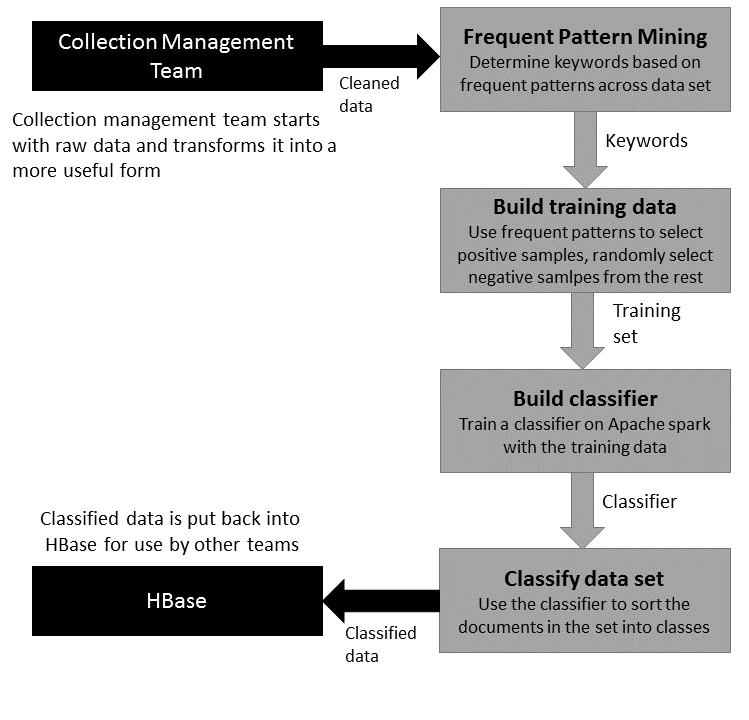
\includegraphics[scale=.65]{figures/design_flow_chart.png}
    \caption{High level overview of the flow of data through the classification system.}
    \label{fig:overview}
\end{figure}

\subsection{Environment Set--Up}
Our group decided to avoid working directly on the cluster, granting us full administrative rights to a machine, which allowed us to set up and test different configurations and algorithms beyond what might currently be supported by the Hadoop cluster being used for class.

A prime example, and the primary motivating factor for our choice, was our decision to use Frequent Pattern Mining (FPM) in the construction of our training sets. The cluster provided for the class was running Spark version 1.2.0, but FPM is not supported by Spark until version 1.5.0. Since FPM was a methodology suggested by the GRAs, and they assured us that they could upgrade the cluster to a more current version of Spark, we decided to proceed with this method.

Due to time constraints, we created a Debian Virtual Machine with sufficient specs to begin writing and testing our methodology. This machine is hosted on a VMware vSphere cluster that belongs to the Virginia Tech IT Security Office/Lab. Since one of the group members works in this lab, we were able to provision this VM. It has been assigned 32 GB of RAM, 16 processor cores, and 40 GB of storage. This has proven to be more than adequate for the testing that we have performed on our small data set.

The Hadoop cluster has since been upgraded to Spark 1.5.0 allowing us to transition our code and methods over and work directly with the HBase instance. As this was a recent change, we are still in the process of this transition and cannot report on what effect it will have, i.e.\ whether there are any issues encountered that break our implementation.

\subsection{Building the Training Data}
In order to begin the classification process we have to prepare a set of training data to use for the machine learning classification algorithm. In order to do this, we assume that we are working with data that has been cleaned of profanity and non-printable characters.

For our methodology we then need to take the content of each tweet and webpage as a string and tokenize it. This means that we will remove any duplicate words and have the result be a set of the vocabulary in the tweet (or webpage). At this stage we also remove any stop words that are in the vocabulary to make sure our algorithms in the next phase are not skewed by taking stop words into account. During this phase we also strip the \# from any hashtags that are present in the tweet.

In our initial design and testing we did not yet have access to cleaned tweets and webpages from the Collection Management team, so we worked primarily to build the methodology that would be used once those resources became available. Therefore, some of the steps mentioned previously, such as the removal of the stop words and the removal of the \# from hashtags are unnecessary when working with the data provided by Collection Management in HBase.

The next step in our algorithm involves the use of Frequent Pattern Mining (FPM) to determine the most frequently used patterns of words in the text of a series of tweets or webpages. FPM looks at the set of existing vocabulary for each text and determines which tokens appear together most often within a tweet's vocabulary.

This is the stage where manual intervention in necessary. We look at a file containing a sorted list of all the frequent patterns; from this we choose a set of features to train on. In our attempts at training a classifier for our small data collection, we chose to select a frequent pattern of four words. This was essentially an arbitrary choice, but we believe that it strikes a good balance between being too specific and missing some relevant tweets and being too broad and pulling in a number of non-relevant tweets.

At this stage we need to create positive and negative training samples. To do this, we pull a random subset of tweets that contain our frequent pattern and classify those as positive samples. For our negative sample we pull a random subset of tweets that do not contain our frequent pattern. To ensure that this labeling is at least mostly correct, we will inspect both the positive and negative training sets (or a portion of them) to confirm that each set is composed of either relevant tweets and webpages or non-relevant ones as appropriate. If in this inspection we find that the choice of frequent pattern has generated a poor training set, we will choose a different frequent pattern and go through the process again.

\foxComment{How long does one iteration take? How big are the training sets? How many iterations are commonly needed?

Add details somewhere.}

%\todo[inline]{Have you checked whether the results of using FPM to determine labeling of tweets as positive or negative is correct?  That is, did you manually check (some) of the label assignments?  Will you use the same approach for webpages too?}For our negative sample we pull a random subset of tweets that do not contain our frequent pattern.

\subsection{Training the Classifier}

We then use the sets of positive and negative samples to train a classifier. We are currently using a logistic regression classifier in our implementation, primarily due to its ease of implementation in Spark.

FPM allows us to develop a training set by filtering the tweets and webpages down to some subset of those that do and do not contain the selected frequent patterns. We take these subsets as the positive training data and the negative training data.

At this point we then feed the selected documents into the classifier; this step uses all the words in each document of the training data, not just the words used for FPM. As we progress we intend to try using several different classifiers to determine which one provides us with the best results.

\foxComment{Remember to give details, along with tables and examples, so your work can be easily reproduced}

%As the project progresses we \todo[inline]{When you try other classifiers, will you use the same training data?  When you use LR and those others, what are the features - just those from FPM, or all words in the labeled documents?}plan to attempt using several different classifiers and comparing their effectiveness at classifying our data.

\subsection{Predicting the Class}

After training the classifier, we apply the classifier to all the tweets across our small data collection. This results in a binary scoring for each tweet as relevant or non-relevant to the collection based upon the training data we selected.

\subsection{Evaluating the Classifier}

We can evaluate the accuracy of our model by judging how well it classifies some of the data that could have been in our positive or negative samples. This is the most intuitive evaluation however it requires a great deal of manual effort to perform. We need to pull out a sampling of classified data and look through it manually, marking whether or not the classification was correct.

Another evaluation that we can perform looks at how well each small collection does at being relevant to the topic at hand. If a large number of the documents in the collection are classified as non-relevant, then the collection as a whole has not done a good job capturing the event in question.

Finally, we need to perform an evaluation of how well our method of using FPM to determine the training documents works. This is much like the first evaluation in that it can be very manual. We will need to dump the generated training sets out to files and then manually decide whether a given set has all (or primarily) relevant or non-relevant documents, as appropriate.


%\todo[inline]{When you mention about not well implemented, does that mean: you are not sure how to do this, you have not done it, you did it but had problems, etc.? Where is the evaluation plan detailed?}We currently do not have this well implemented, but plan to have this evaluation completed before the next report.

\subsection{Interfacing with HBase}

\subsubsection{Manual File Uploading}

We are currently able to process the six small data files and determine a probability representing how likely it is that a specific tweet is relevant to the collection. For each of the data sets we have produced a .tsv file with two columns: one containing the tweet ID (which serves as the row key in HBase), and one containing a value between 0.0 and 1.0 which represents the probability that the tweet is relevant to the category. 

Within HBase, we have created a column family named "classification." Within our column family, we only have need of one column, named "relevancy." This column is where the probability value for each document in the database will be stored for access by other teams. Figure \ref{fig:hbase-data} shows an example query for a row, which returns all of the data in that row. The data produced by our system is highlighted.

\begin{figure}[ht]
	\centering
	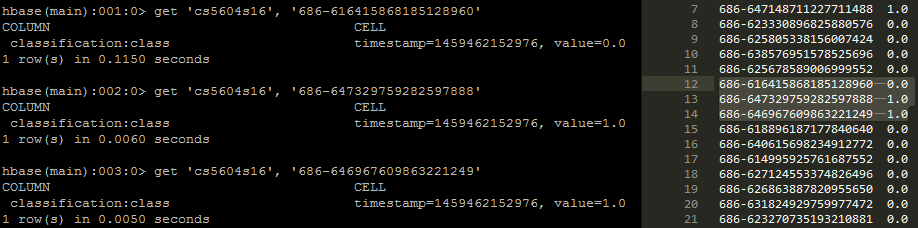
\includegraphics[scale=.65]{figures/hbase-data.png}
    \caption{An example row in HBase. Our data is highlighted.}\label{fig:hbase-data}
\end{figure}

For this version of the system, we are inserting the data into HBase manually. We accomplish this by using Hadoop's importTsv script as explained in the tutorial provided by the Solr team. The importTsv script is provided by HBase and allows you to take a .tsv file and specify what the columns in the file contain. We accomplish this with the following command:

\begin{lstlisting}[language=bash]
 $ hbase org.apache.hadoop.hbase.mapreduce.ImportTsv \
   -Dimporttsv.columns=HBASE_ROW_KEY,classification:relevance \
   ideal-cs5604s16 DATA_FILE
\end{lstlisting}

Here you can see we specify in the "-Dimporttsv.columns=" parameter that the first column in our .tsv file corresponds to the row key and the second corresponds to the classification:relevance column. We also specify that we are writing to the "ideal-cs5604s16" table and give it the file to upload.

\subsubsection{Direct Reading and Writing}

Using the importTsv script has allowed us to work on our system in our own virtual environment, since we are able to produce output files that can then be manually uploaded to the cluster. This was very useful while we were waiting for the software on the cluster to be updated so that we would have access to necessary libraries. Now that the software on the cluster has been updated, we are moving our implementation on to the cluster and making it so that our classification system will directly read data from and write data to the database.

Directly reading and writing from the database has several advantages. The main advantage and the primary motivation for doing it this way is that it will allow us to automate the process. Our system will be able to work directly with the HBase table, and will not need someone to manually feed it data files as input and handle the files it produces as output. This will greatly simplify the classification process for any future data that gets added to the database.

Directly reading and writing from HBase is done via the pyspark library provided by Spark. The library allows python to establish a connection to HBase which it can use to stream data back and forth. We currently have a rudimentary "hello world" version of this process working on our local virtual environment. We are working towards moving the implementation to the cluster and adapting it to read and write from the "ideal-cs5604s16" table. This functionality will be complete by the final report.

% Here is the introduction. The next chapter is chapter~\ref{ch:ch2label}.


% a new paragraph


% \section{Examples}
% You can also have examples in your document such as in example~\ref{ex:simple_example}.
% \begin{example}{An Example of an Example}
%   \label{ex:simple_example}
%   Here is an example with some math
%   \begin{equation}
%     0 = \exp(i\pi)+1\ .
%   \end{equation}
%   You can adjust the colour and the line width in the {\tt macros.tex} file.
% \end{example}

% \section{How Does Sections, Subsections, and Subsections Look?}
% Well, like this
% \subsection{This is a Subsection}
% and this
% \subsubsection{This is a Subsubsection}
% and this.

% \paragraph{A Paragraph}
% You can also use paragraph titles which look like this.

% \subparagraph{A Subparagraph} Moreover, you can also use subparagraph titles which look like this\todo{Is it possible to add a subsubparagraph?}. They have a small indentation as opposed to the paragraph titles.

% \todo[inline,color=green]{I think that a summary of this exciting chapter should be added.}